\chapter{Implementing Socrates Sim}
\label{chap:implementation}

\section{Overview}

In this chapter, we describe how to implement and deploy Socrates Sim. We first describe the general process of setting up Socrates Sim. In chapter \ref{chap:restaurant} and chapter \ref{chap:movie}, we focus specifically on the implementation choices and details for supporting the restaurant recommendation and movie booking domains. These domains were chosen for different strategic reasons. The restaurant domain was selected due to the availability of training data from the Dialog State Tracking Challenge 2 (DSTC2). The dialog acts and slot values are well defined by the organizers of DSTC2. We had to manually scrape restaurant data from Yelp in order to build out the database of restaurants to use for recommendations. We used the training dialog data to train the neural translation models to support model based natural language understanding (NLU) and natural language generation (NLG). 

 The movie booking domain was selected so that we could run performance tests against the TC-Bot framework \cite{li_end_to_end}. TC-Bot was hardcoded to support the movie booking use case. While the TC-Bot code repository provided some domain configuration data, it was ultimately unusable. As a result, we defined a new but analogous domain and manually created a new movie database. As there was no dialog data available for training, we did not implement model-based NLU and NLG components for the user simulator. Instead, we used a rules-based approach. 
 
Please note, we refer to the end user as the researcher, as that is the presumed user of our framework. We aim to demonstrate the value of Socrates Sim directly though applied examples. 

\section{General Process to Deploy Socrates Sim}

The Socrates Sim framework is domain and speaker agnostic. All domain, dialog agent, and user simulator specifics have been abstracted away. Therefore the researcher must inform Socrates Sim about the dialog domain and where the speaker classes are located. Prior to running Socrates Sim, the researcher has to prepare the components required to run a simulation. At a high level, the researcher needs to: 
\begin{itemize}
	\item Define the dialog domain 
	\item Develop the interface classes for the user simulator
	\item Develop the interface class for the dialog agent
	\item Define the simulation settings
\end{itemize}

The researcher then can invoke Socrates Sim to run multiple simulations and generate train data. Next, we will briefly explore how to implement the components above. We further explore domain specific implementation details in the proceeding chapters. 

\subsection{Defining the Dialog Domain}

The first thing the researcher should do is define the dialog domain. The dialog domain captures the various dialog acts, inform and request slots, slot values, and other information pertinent to their domain. Domain information is formally captured and represented to Socrates Sim as a \textit{domain} object (see section \ref{sssec:dialog_domain}). This object is made available to the user simulator, dialog agent, and dialog manager. The object is static and does not change in order to ensure consistent communication between all parties. 

The researcher does not need to manually create and instantiate the domain object. All the domain information is captured in a yaml or json configuration file (e.g. Figure \ref{fig:sample_domain}). The yaml format is recommended for small domains that can easily be written out by hand. For larger complex domains, the json format is recommended as it is easier to export programmatically. 

\begin{figure}[h!]
	\centering
	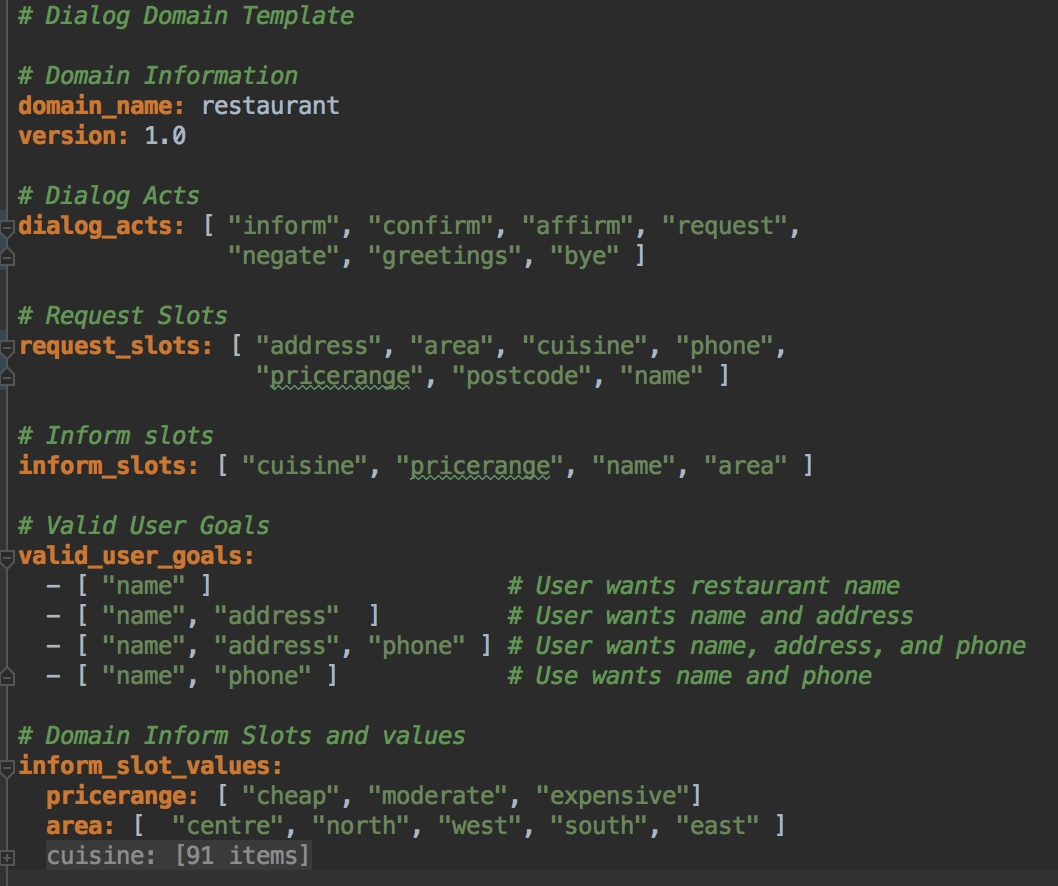
\includegraphics[scale=.25]{diagrams/sample_domain.jpeg}
	\caption{ Sample domain configuration file. }
	\label{fig:sample_domain}
\end{figure}

As seen above, the dialog information is captured with key-value pairs. The values in most cases are lists of items (e.g. a list of valid dialog acts). Inform and request slot values are represented as nested dictionaries. Each slot is a nested key that points to a list of valid slot values. Chapter \ref{chap:design} specifically outlines the various domain attributes. The one thing it does not cover is the valid user goals. 

Valid user goals are an optional piece of information the researcher can provide to Socrates Sim. At the beginning of each round, the dialog manager will generate a goal for the user simulator. This goal can be randomly selected from a preexisting list of valid goals or randomly generated from the request and inform slot information in the domain object. In the valid user goals section, the researcher lists the different combinations of valid request values that can be used when generating a goal. This is to ensure the random goal generator does not generate a user goal with no request slots (implying the user has no goal in mind) or accidentally select request slots that produce invalid goals.  

Additionally, the researcher may have a knowledge base that they want to provide to the dialog agent. The knowledge base can be used by the dialog agent to make suggestions. We create a simple interface to allow the dialog agent to access information from a knowledge base in a standardized way. The \textit{DomainKBTable} class will take in a csv file and convert it into a pandas data frame. It additionally provides a set of query and sampling methods. The \textit{DomainKBTable} object is a public property of the domain class.

At runtime, the dialog domain information stored in the configuration file is dynamically loaded and converted into \textit{domain} object by the run script. For local testing, the researcher can invoke the \textit{import\_domain} method from the \textit{dialog\_simulator} module to manually instantiate the object. 

\subsection{User Simulator and Dialog Agent  Interface}
\label{sec:speake_interface}
The process for integrating an external user simulator and dialog agent into Socrates Sim is very similar. The researcher needs to create an interface class that allows Socrates Sim to communicate with both speakers in a standardized manner.  This is accomplished by creating a subclass of the base \textit{UserSimulator} and \textit{DialogAgent} (see Figure \ref{fig:speaker_ext}). Both these base classes are implementations of the \textit{Speaker} abstract base class described in section \ref{sssec:speaker}. 

\begin{figure}[h!]
	\centering
	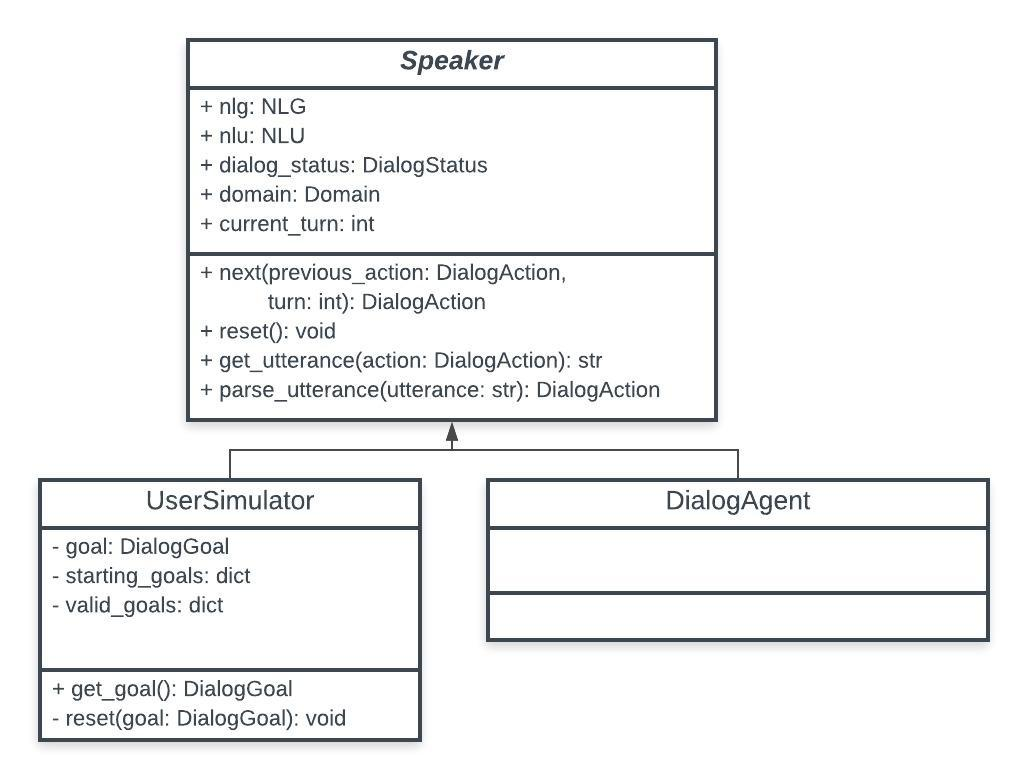
\includegraphics[scale=.75]{diagrams/speaker_classes.jpeg}
	\caption{ Extending Speaker class for user simulator and dialog agent.} 
	\label{fig:speaker_ext}
\end{figure}

The key distinction between both base classes is the requirement of transparency for the user simulator. The framework assumes that the dialog agent is opaque and can only communicate with the framework through dialog action objects. Therefore the \textit{DialogAgent} serves more as a template for implementation.  In contrast, the user simulator is required to be more transparent and accessible in a particular manner by the dialog manager. At the beginning of each round, the dialog manager generates a user goal and updates the user simulator with that goal. Additionally, at the end of each conversation round, the internal state of the user simulator's goal is extracted and stored in the dialog history that is actively tracked by the dialog manager. As a result, the researcher must implement get\_goal and override the reset methods in addition to the interface methods defined in the \textit{Speaker} abstract base class. The dialog goal is formalized as a \textit{DialogGoa}l object and more details about it can be found in section \ref{sec:dialog_goal}. 

Both the user simulator and dialog agent interface subclasses must implement the following methods: \textit{reset}, \textit{next} \textit{get\_utterance}, and \textit{parse\_utterance}. The method signatures and return types are strictly defined and enforced to ensure that both speakers communicate with Socrates Sim in a standardized manner. As Python is a dynamically typed language, we use the type hinting feature introduced in Python 3.5 to signal to method contracts and expectations. 

The \textit{reset} method is used to reset the internal state of the speaker. That is, all inform/request slots are cleared and any internal state tracking is set back to 0. It is called by the dialog manager at the start of each simulation round. The \textit{reset} method of the user simulator is also expected to take in a dialog goal object, which is generated anew by the dialog manager. 

The \textit{next} method is the critical method that drives the simulation. It is used to capture the current speaker's response to its interlocutor. The \textit{DialogAction} class is central to standardizing communication between the speakers and the dialog manager. Each speaker must produce a dialog action object that captures both the raw speech utterance and its semantic representation. The specific design of the \textit{DialogAction} class can be found in section \ref{sssec:dialog_action}. The \textit{next} method takes in as input the dialog action of the previous speaker and the current turn number. It outputs the current speaker's response as a new dialog action object.

Finally, the \textit{get\_utterance} and \textit{parse\_utterance} methods are tied directly to the speaker's internal \textit{NLU} and \textit{NLG} objects. The \textit{parse\_utterance} method will take in a natural language speech utterance and pass it directly to the speaker's internal nlu object for parsing. The \textit{parse\_utterance} method will then output a new dialog action object with the parsed semantic frame representation of the utterance. The \textit{get\_utterance} does the reverse of \textit{parse\_utterance}. It generates a speech response from a provided semantic frame representation. The internals of how the nlg and nlu objects are defined is up to the researcher. In the restaurant use case, we explore how to use a rules-based and a model-based strategy. It is important to note that the researcher can specify the \textit{NLU} and \textit{NLG} class implementations in the simulation file. By abstracting out the nlu and nlg process from the speaker's internal logic, we support the ability for experimentation and code reuse. 

\subsection{Simulation Configuration}
After the researcher has prepared all the requisite components for using Socrates Sim, they need to capture that information in a configuration file.  Specifically, the researcher has to provide Socrates Sim with the following: the path to the domain configuration file, the path to the user simulator class, the path to the dialog agent class, and the simulation settings. This information is collected in a yaml or json configuration file that is provided to Socrates Sim at runtime (see Figure \ref{fig:sample_sim_config}). 

\begin{figure}[h!]
	\centering
	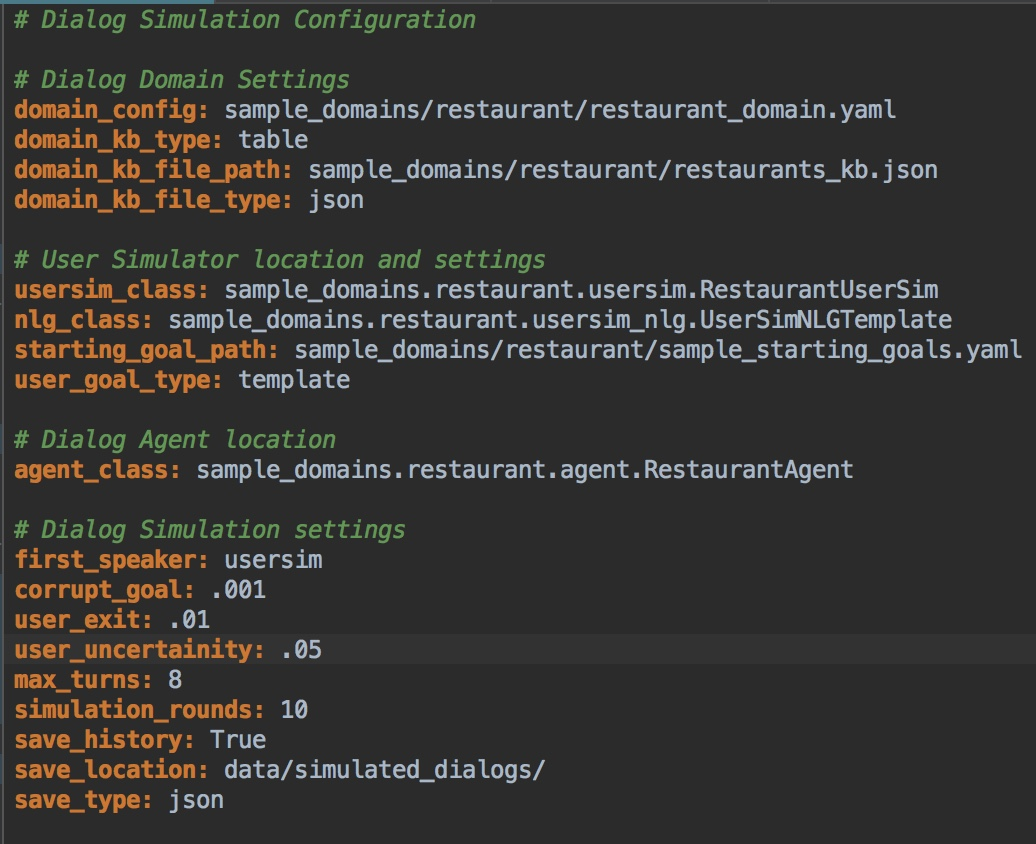
\includegraphics[scale=.25]{diagrams/sample_sim_config.jpeg}
	\caption{ Example simulation configuration file. }
	\label{fig:sample_sim_config}
\end{figure}

The researcher also specifies the various simulation settings (e.g. number of simulations to run, where to store generated dialogs, etc). Figure \ref{fig:sim_settings} outlines out the various settings supported by Socrates Sim.

\begin{figure}[h!]
	\centering
	 \begin{tabular}{|l|p{5cm}|p{5cm}|}
		\hline 
		\textbf{Setting} &\textbf{ Description } & \textbf{Valid Values } \\ 
		\hline 
		first\_speaker & Defines who speaks first  & user, agent, random  \\ 
		\hline 
		corrupt\_goal & Probability the user's goal is randomly corrupted resulting in random user behavior  & valid probability in range [0.0, 1.0]  \\ 
		\hline 
		user\_exit & Probability user randomly exits conversations  & valid probability in range [0.0, 1.0]  \\ 
		\hline 
		user\_uncertainty & Probability user randomly changes mind and goal  & valid probability in range [0.0, 1.0]  \\ 
		\hline 
		max\_turns & Maximum amount of conversation turns before simulation is aborted.  &  Reasonable real integer greater than 0 \\ 
		\hline 
		simulation\_rounds & Number of simulations to run.  &  Reasonable real integer greater than 0 \\ 
		\hline 
		save\_history & Flag to indicate if generated dialogs should be saved & True or False  \\ 
		\hline 
		save\_location & Location to store generated dialogs  & valid save path  \\ 
		\hline 
	\end{tabular} 
	\caption{ Supported simulation settings.}
	\label{fig:sim_settings}
\end{figure}

We made a deliberate choice to adopt a configuration file first approach to communicate settings and other information to our framework. We drew inspiration from \cite{Gardner_allennlp}, which uses configuration files for the communication of model details and experiment parameters to the AllenNLP framework. In traditional command line tools, parameters are passed to the tool by command-line arguments. For example, Figure \ref{fig:cmd_line_ex} contains the command line parameters to run 300 simulations on the TC-Bot simulators. 

\begin{figure}[h!]
	\centering
	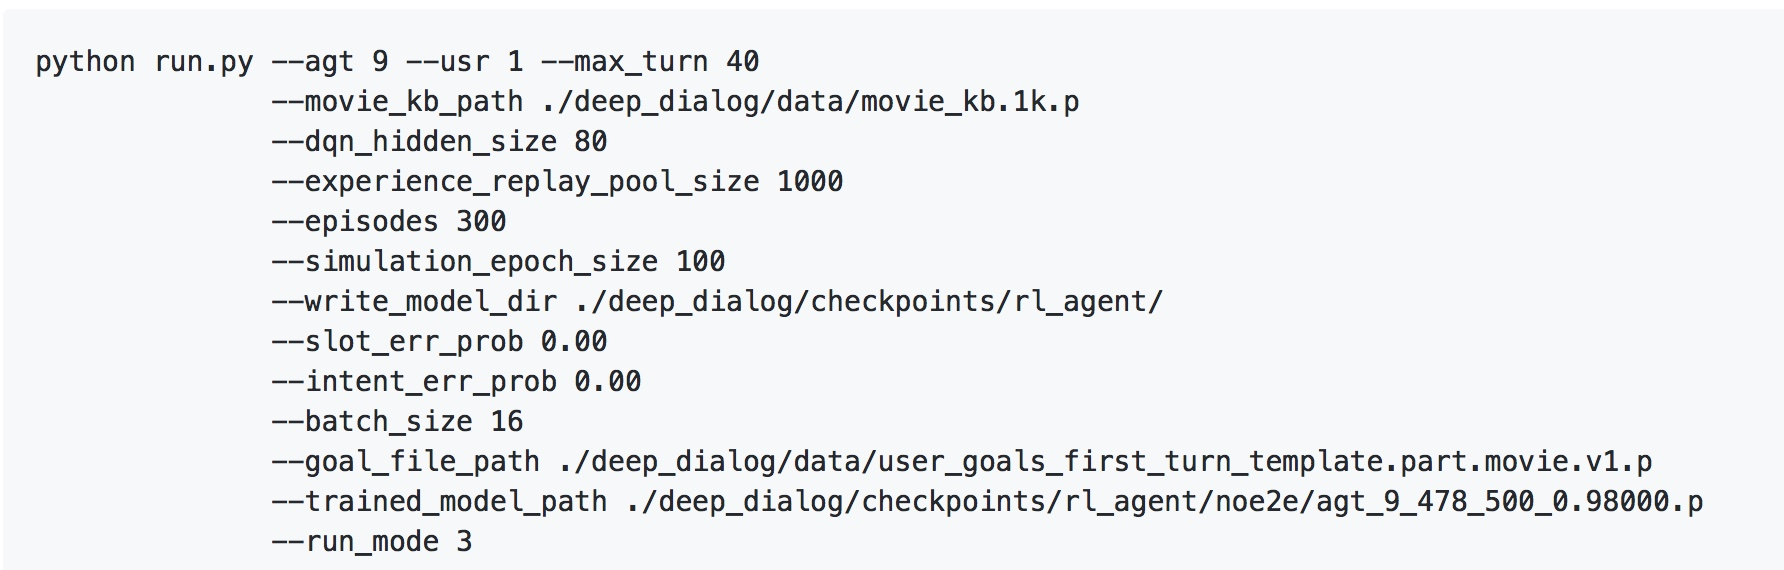
\includegraphics[scale=.25]{diagrams/cmd_line_ex.jpeg}
	\caption{ Command line parameters to run 300 simulations with TC-Bot. }
	\label{fig:cmd_line_ex}
\end{figure}

The challenge with this approach is that command line invocation can grow more complex as more parameters are added. Long invocation commands needs to be carefully formatted to ensure there are no line breaks and proper spacing is observed to separate out the arguments. This often results in a poor user experience. It is cumbersome to remember and cleanly enter all the information required each time the program is run. In practice, most users end up creating a reference file from which they copy and paste the command line statement. Socrates Sim supports both json and yaml formatted configuration files. Yaml is the recommended format as it is more human-readable and is easy to write. If the researcher wants to generate configuration files as part of a larger pipeline or does not like yaml, the json format is also supported. 

\section{Simulating Dialogs with Socrates Sim}

The last step in the process is actually running Socrates Sim and generating simulated dialogs. The framework is implemented as a command line tool. The user invokes a run script with the location of the simulation configuration file. If the researcher chooses to save the output, the generated dialogs will be serialized as a json file. Additionally, the researcher can signal Socrates Sim to print the simulation in a terminal using the \textit{-pd} flag. 

\begin{figure}[h!]
	\centering
	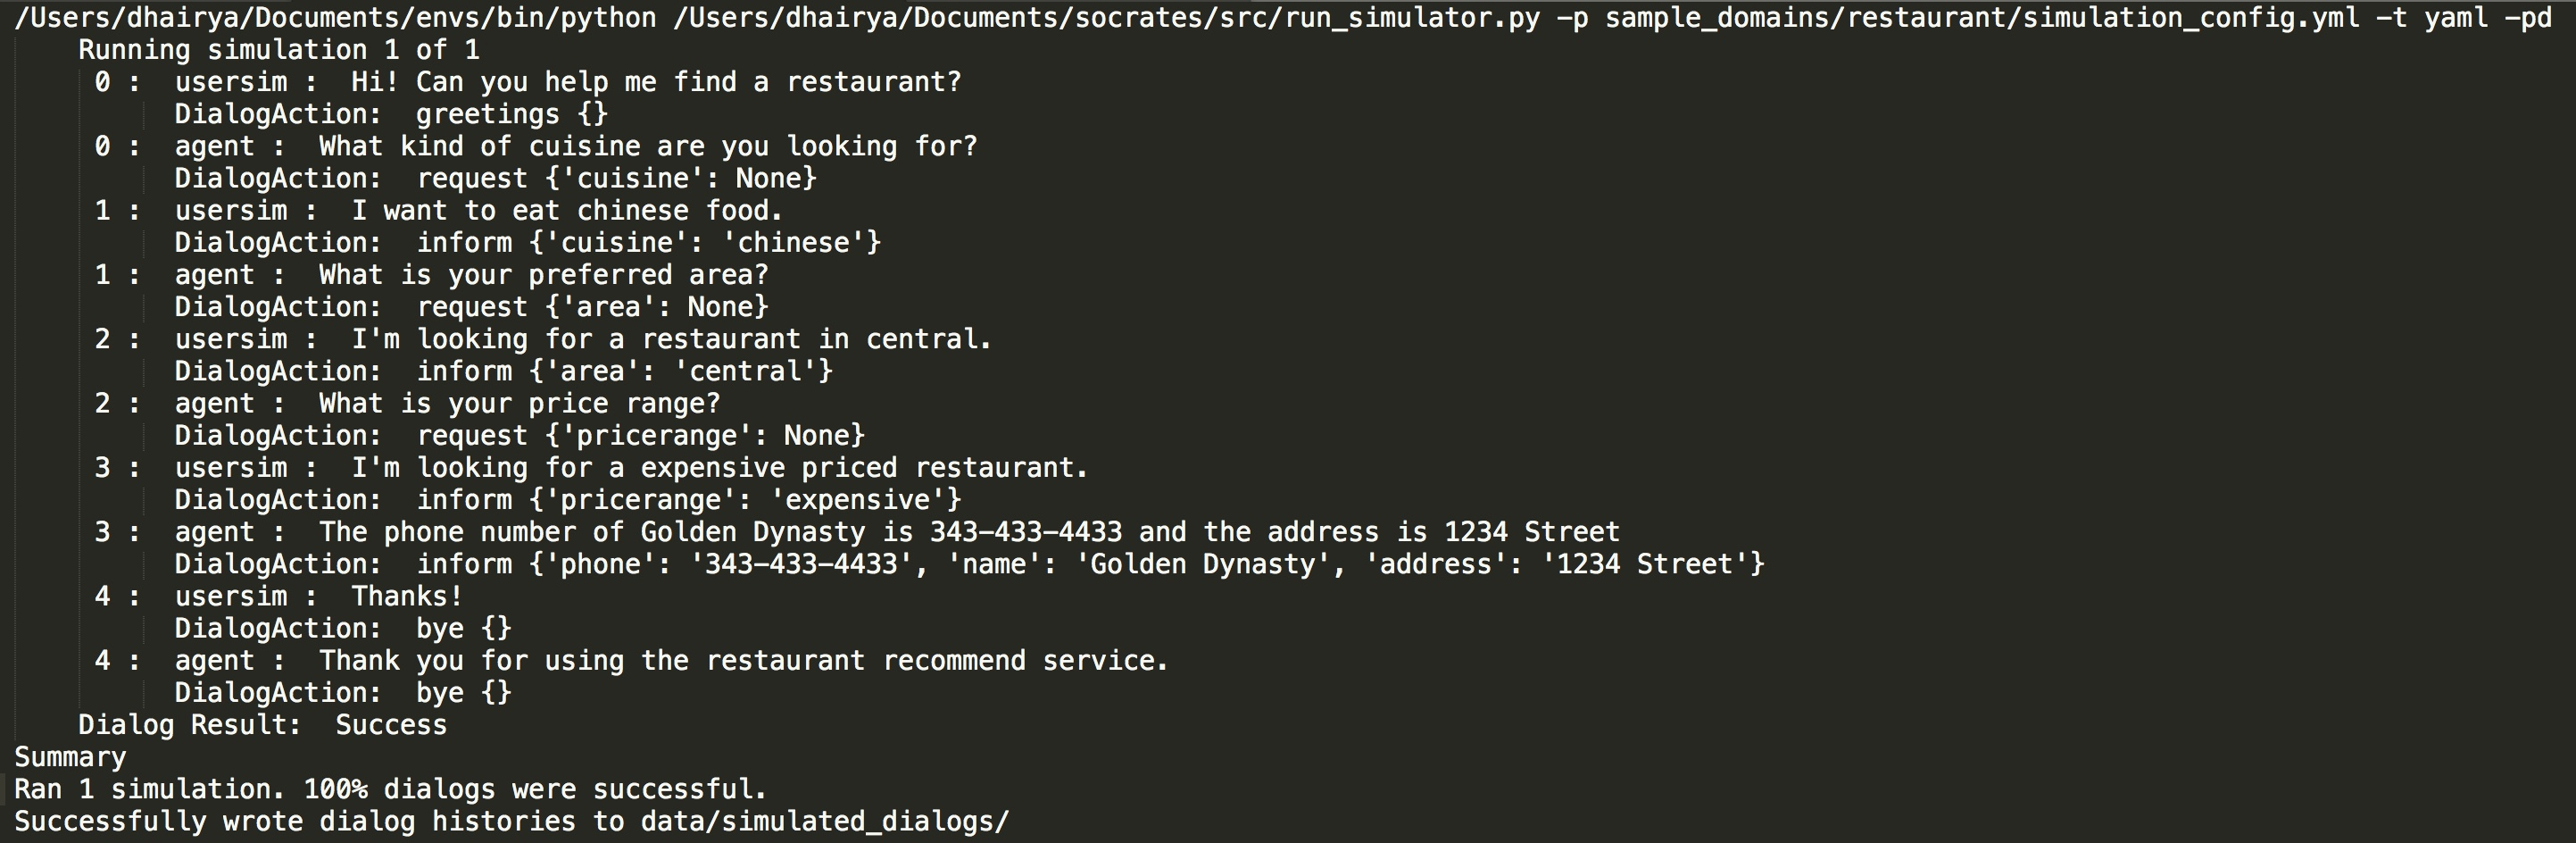
\includegraphics[scale=.15]{diagrams/sample_run.jpeg}
	\caption{ Sample run of the Socrates Sim framework. }
	\label{fig:sample_run}
\end{figure}

Behind the scenes, the run script first loads in the simulation configuration file. Next, it initiates the dialog manager and passes along all the simulation settings. The dialog manager first loads the various components (reading in the dialog domain, initializing the interface classes for the user simulator and agent, etc). Next, it starts the simulation process and facilitates the various conversations between the user simulator and dialog agent. At the end of each conversation round, the dialog manager evaluates the conversation based on the end state of the user simulator's goal object. If all the request slots in the goal object are filled, the dialog manager grades the simulation as successful. 

\begin{figure}[h!]
	\centering
	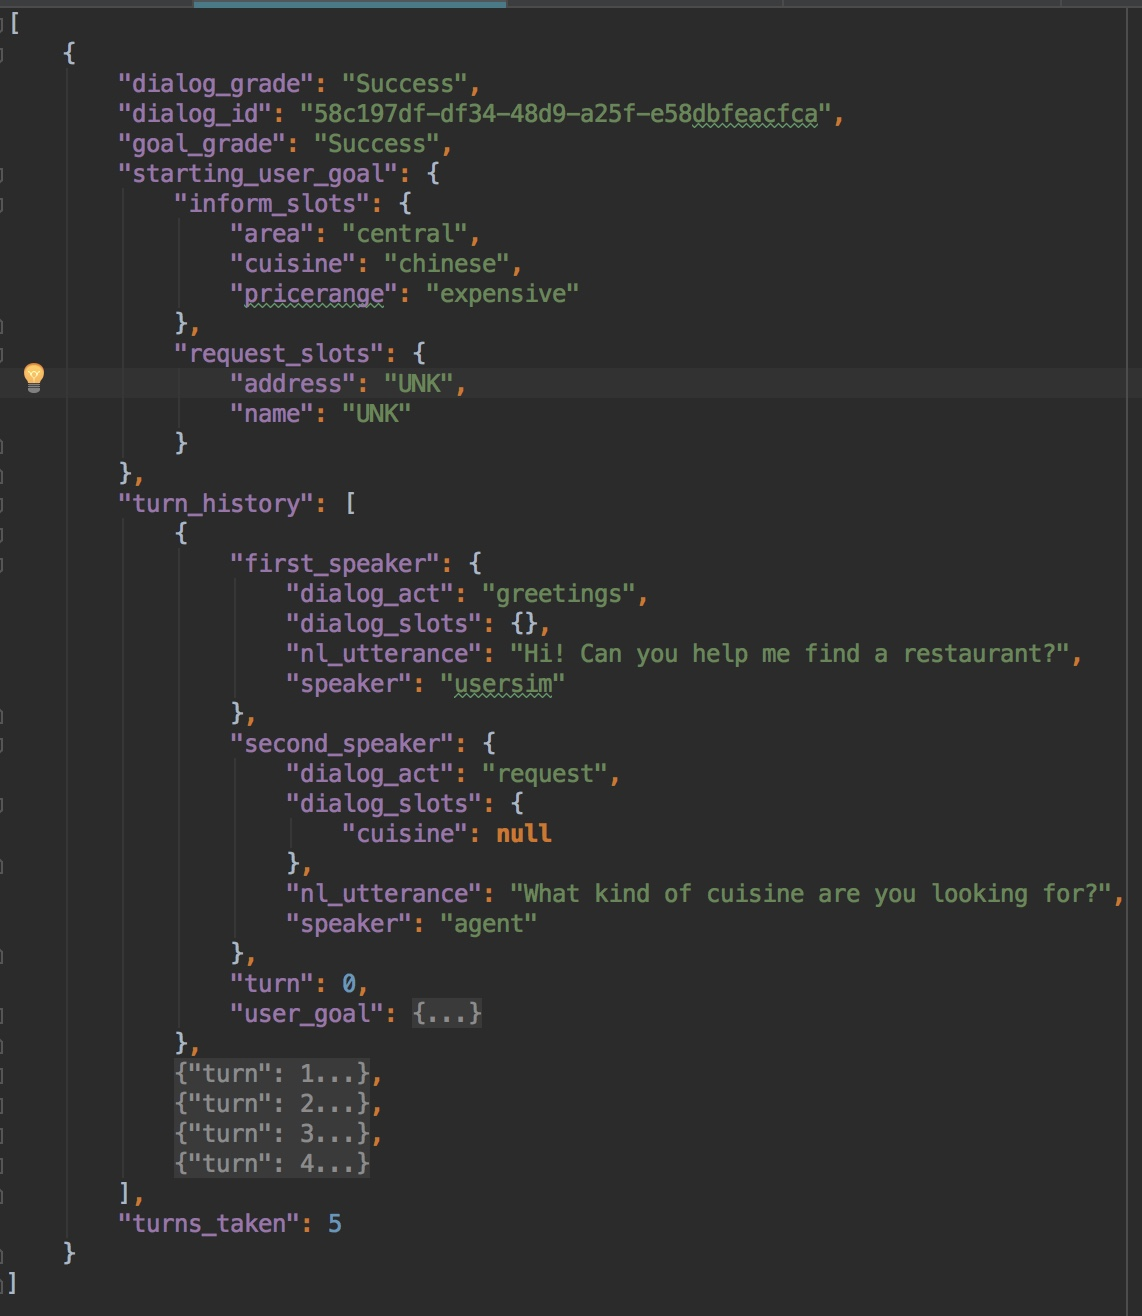
\includegraphics[scale=.17]{diagrams/sample_save_output.jpeg}
	\caption{ Sample output after running one simulation round. }
	\label{fig:sample_output}
\end{figure}

After all simulations have been run, the dialog manager will serialize the output (if specified by the researcher) and exit. Figure \ref{fig:sample_output} shows an example output generated after running one simulation. The goal of the output file is to provide quality annotated data that can be used as training data for supervised learning or reinforcement learning based dialog agents. The output contains several pieces of key information. Each simulation is assigned a unique id, information about the number of turns taken, the grade of the simulation, the user's initial starting goal, and turn history, which contains the annotated history of the conversation round. 

Socrates Sim is written to be extensible. Given its modular nature, the researcher has the ability to extend the framework to support new use cases. Next, we show how Socrates Sim was adapted for the restaurant and movie domains. 

%%% Local Variables: 
%%% mode: latex
%%% TeX-master: "main"
%%% End: 

